\documentclass[9pt,twocolumn,twoside]{pnas-report}

\templatetype{pnasresearcharticle}

\usepackage{lipsum}
\usepackage{mathtools}
\DeclarePairedDelimiter\floor{\lfloor}{\rfloor}

\title{Effect of Key Match Events on Football Passmaps}

\author[a,1]{Vid Stropnik}
\author[a]{Vuk \DJ uranović}
\author[a]{Maruša Oražem} 


\affil[a]{University of Ljubljana, Faculty of Computer and Information Science, Ve\v{c}na pot 113, SI-1000 Ljubljana, Slovenia}


\leadauthor{Stropnik} 
\authordeclaration{All authors contributed equally to this work.}
\correspondingauthor{\textsuperscript{1}To whom correspondence should be addressed. E-mail: vs2658@student.uni-lj.si}





\begin{abstract}
\lipsum[1]
\end{abstract}

\dates{The manuscript was compiled on \today}
\doi{\href{https://ucilnica.fri.uni-lj.si/course/view.php?id=183}{Introduction to Network Analysis} 2020/21}

\begin{document}

\maketitle
\thispagestyle{firststyle}
\ifthenelse{\boolean{shortarticle}}{\ifthenelse{\boolean{singlecolumn}}{\abscontentformatted}{\abscontent}}{}



\dropcap{A}{\bf ssociation football is the world's most popular sport.} During gameplay, players attempt to create goal-scoring opportunities through various methods of individual control of the ball. While these can include dribbling, tackling and taking direct shots, the most common one is passing the ball to a teammate. Progressing the ball along the pitch with a series of passes helps the team retain control of the match, enabling them to realize set plays. It is worth noting that this method is not only common, but also effective, as exhibited by the correlation of per-game average pass frequency and overall tea, success. \cite{plpasses}

Ball movement and goal-scoring opportunities in a football match are complex phenomena to model. Pass characteristics, such as their length, speed or the involved players' positions are often used to provide further insights into their importance and quality. Logging such characteristics for hundreds of passes that happen in any given football match, however, renders the resulting data structure very complex and hard to interpret. To infer more general information about longer stints of play, simpler arrangements, such as networks with player nodes and directed pass links, should be considered.

There are several events in any given football match, that might incur a fundamental change in a team's tactics and approach towards the game. The coaching staff might recognize weak points in the opposition's strategy and relay them to the players during half-time. Suddenly conceding a goal in a must-win game might prompt a team to take more risks and try a different approach, while we can often observe leading teams resort to time-wasting tactics to ensure their victory. 

In this course project, we introduce novel ways of football match analysis using established network science approaches. By using methods of measuring change in team pass map centrality, by observing alterations of its underlying communities and by recognizing the (dis)appearance of distinct player graphlets as a result of a key event in a football match, we study common team behaviours that key match events might induce. We recognize these insights as useful in several areas. First, they serve as a form of establishing several ground truths about common trends of play, that will underpin further research. Secondly, more fine-grained difference of successful and unsuccessful responses to key events might be observed and be used in match preparations by domain experts. Finally, we recognize real-time applications of the proposed methods as useful in broadcasting, betting, commentary and analytics, to name only a few fields.

This report is structured as follows: In the following paragraphs, we provide a brief overview of the work, relating to inferring insights from sports data using network analysis. Here, we also introduce some key academic contributions to our work in the tree network science fields of special interest: measuring centrality, detecting communities and gathering semantic information from network graphlets. A subsection corresponds to each of these fields in the succeeding \textit{Results} section. In them, we introduce the main revelations about the effects of key match events on passing trends. We later comment on the implications of these results and asses their appropriateness for further application, while finally introducing our detailed methodologies at the end of the paper.



%\begin{figure}[t]\centering%
%	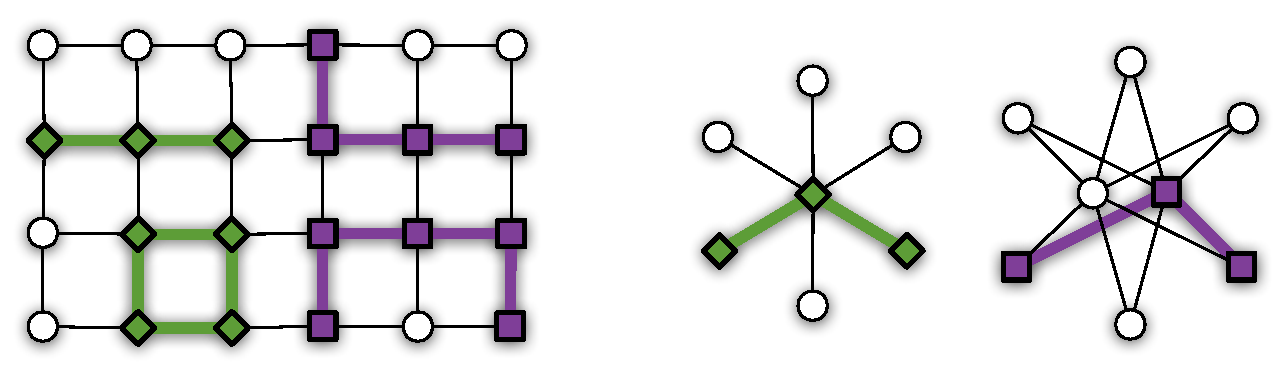
\includegraphics[width=0.8\linewidth]{examples}
%	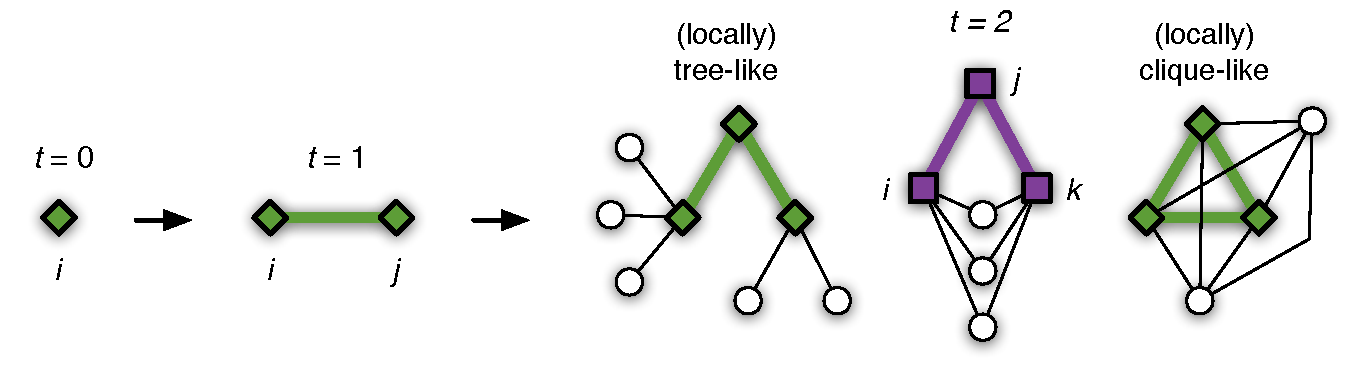
\includegraphics[width=\linewidth]{growth}
%	\caption{Mandatory informative illustration highlighting main %contributions.~\cite{Sub18a}}
%	\label{fig:example}
%\end{figure}

\section*{Related work}
Evaluations of group performances based on their underlying network structures have been conducted for some time. Researchers were keen on understanding what kind of social, interaction or communication network structure boosts the productivity of a group in a working environment. Bavelas \cite{bavelas} was one of the pioneers in exploration of information transfer between groups. He discovered that the rate of information diffusion was significantly smaller in decentralized networks in comparison to centralized ones. It was later discovered by Shaw \cite{shaw} that this gave an edge to decentralized groups over the centralized ones in solving complex tasks. \

Team performance in collective sports has become a well researched area in the network analysis community in recent years. We recognize the conclusions by Grund \cite{grund} as a good starting point for the study of this field. In his work, he suggests that small networks (i.e. the eleven-node football team) are better explained with the use of the weighted edges between players. In such cases, weights are determined by the frequency of passes between two players. He also introduces a measure called network intensity, as a counterpart to network density in large and unweighted networks. This measure is computed as a function of weights for each link between players, nicely called the passing-rate of the team. As a result of his work, Grund confirmed that an increase in team passing rate leads to increased performance, while increases in centralization of play reduces team performance. Similarly to our work, network metrics were used to examine differences between halftimes in work by Clementine {Clementine}, albeit with a different form of pass-map representation.  The authors of \cite{duch2010quantifying}, again envisioned a football match as a weighted directed network, where they introduced a node measure called flow centrality - a function of pass accuracy and ratio of times a player was included in an action, leading to a shot on goal. Using it, they successfully graded individual player performances within a team. The measure is based on betweenness centrality, which has also been applied to football matches to examine correlations of physical demands in elite football players \cite{castellano2019network}. While these works' conclusions are introduced as solid and objective, the importance of considering additional meta-data in the inference of flow using centrality measures was emphasized in the traffic domain in \cite{kazerani2009can}.

While several graphlet and motif-related methodology in our work is heavily inspired by the work of Pržulj \cite{przulj}, the concept of network motifs, initially shown by Milo et al. \cite{Milo}, has been successfully applied to sporting pass-maps by other authors as well. Notably, Penna and Touchette \cite{penna} analyzed the network motifs to analyze passing behaviour, while Bekkers and Shaunak \cite{Bekkers} use meta-data equipped motifs (Possession Motifs and Expected Goal Motifs) to answer more in depth domain questions and graphically visualize team or player similarity by means of radar graph.

Due to advances in player-tracking technology, most recent research, such as those by Fernandez and Born \cite{fbrn}, or by Chawla et al. \cite{chawla}, exploits the spatial-temporal data about observed passes. Due to time restrictions, posed by the gathered data, we don't consider these additional pieces of information in our analysis, but instead focus on the starting formation of the team in determining the positions of players. Researchers opting for the former approach of inferring information from additional metadata, however, should also consider work by Mattson and Takes \cite{trajectory} on pass trajectory extraction. Spatio-temporal methods are also successfully applied to football to accurately detect individual player behaviour and changes in team formation. \cite{bialkowski2014large}.

\section*{Results}

\subsection*{Centrality and intensity}
\subsection*{Communities}
\subsection*{Network fragments}
Another popular technique for inferring global and local network information is the analysis of its fragments. The concept of these induced subgraphs (motifs) and the roles (orbits) individual players represent within them, translates well to the consideration of a sports team's passing map.\footnote{Given that three to four player interlinks have been popularized both in pop culture and academia \cite{triangle}, with perhaps the most prominent representative being the infamous Triangle offence in American basketball.}  Using these techniques, individual team performances may be profiled using numbers of orbit-occurences-per-player (OPP) or motif significance approaches. These, also visualized in Figures \ref{fig:BarcaOPP} and \ref{fig:Barca Significance}, offer a concise way of understanding differences between two passmaps - in these instances, from the same match. Combined with the knowledge of the chosen motif and orbit labelling conventions, here provided in Figure \ref{fig:Motifs}, such plots can be efficiently used to garner insights into the teams' dynamics. 

\begin{figure}[t]\centering
	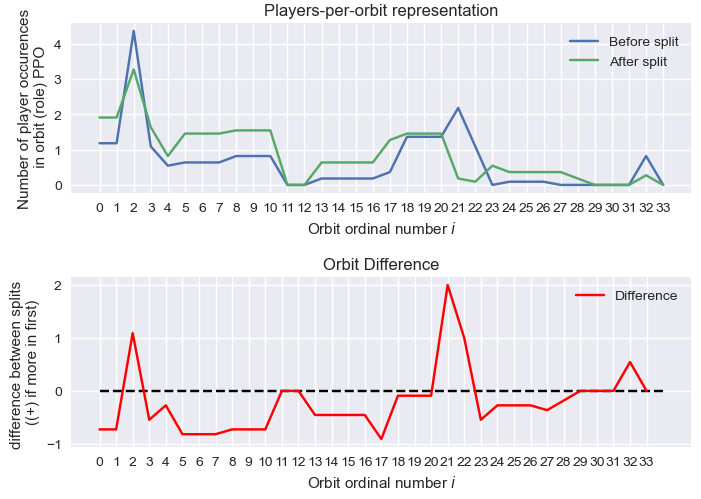
\includegraphics[width=\linewidth]{barcaopp.png}
	\caption{The Orbit-occurence-per-player profile plots for Barcelona's 2017/18 victory over Real Madrid. The graph shows comparison between the two halves. We can see that the number of players occuring in the orbit number 21, as seen in figure \ref{fig:motifs} significantly decreased in the second half.}
	\label{fig:BarcaOPP}
\end{figure}

\begin{figure}[t]\centering
	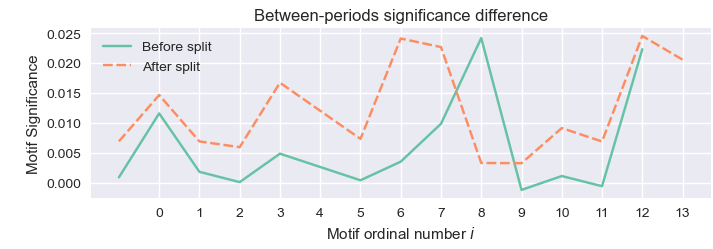
\includegraphics[width=\linewidth]{barcasignif.png}
	\caption{The motif significance profile for Barcelona's 2017/18 victory over Real Madrid. From the graph, we can discern that the abundance of observed motifs \textit{8} played a significant role in characterizing the first half, whereas there was a general increase in the significance of lower-order motifs in the second half.}
	\label{fig:Barca Significance}
\end{figure}


Certain motifs characterize football ball movements better than others. In our general testing, as part of which we showed that no special change is induced by the half-time key event, we established the most notable ones to be the 0th, 7th, 8th and 13th. For all said motifs the median significance z-score exceeded the 3 standard deviations. Perhaps more interesting is the motif significance behaviour when observing the effect of a player-dismissal on a match. In expectation, the number of occurences of the 9th motif will actually reduce significantly below the number of those emerging from random 10 node configuration graphs. Along with this insight, Figure \ref{fig:MotifSignificanceDismissal} also shows that the punished's opposition will actually attempt to exploit their numeric advantage using these most significant playing patterns \footnote{Due to dismissals usually happening late in the analyzed graphs, not enough data was gathered to infer the correct significance of the 13th component, while it additionally being really rare in configuration model networks.} This approach, and the analysis of orbits, provbe to be somewhat interchangable. Consider, for example, that the most significant nodes coincide with the orbits in which we can observe most key match event differences, such as those in Figure \ref{fig:OrbitGoals}.
 
\begin{figure}[t]\centering
	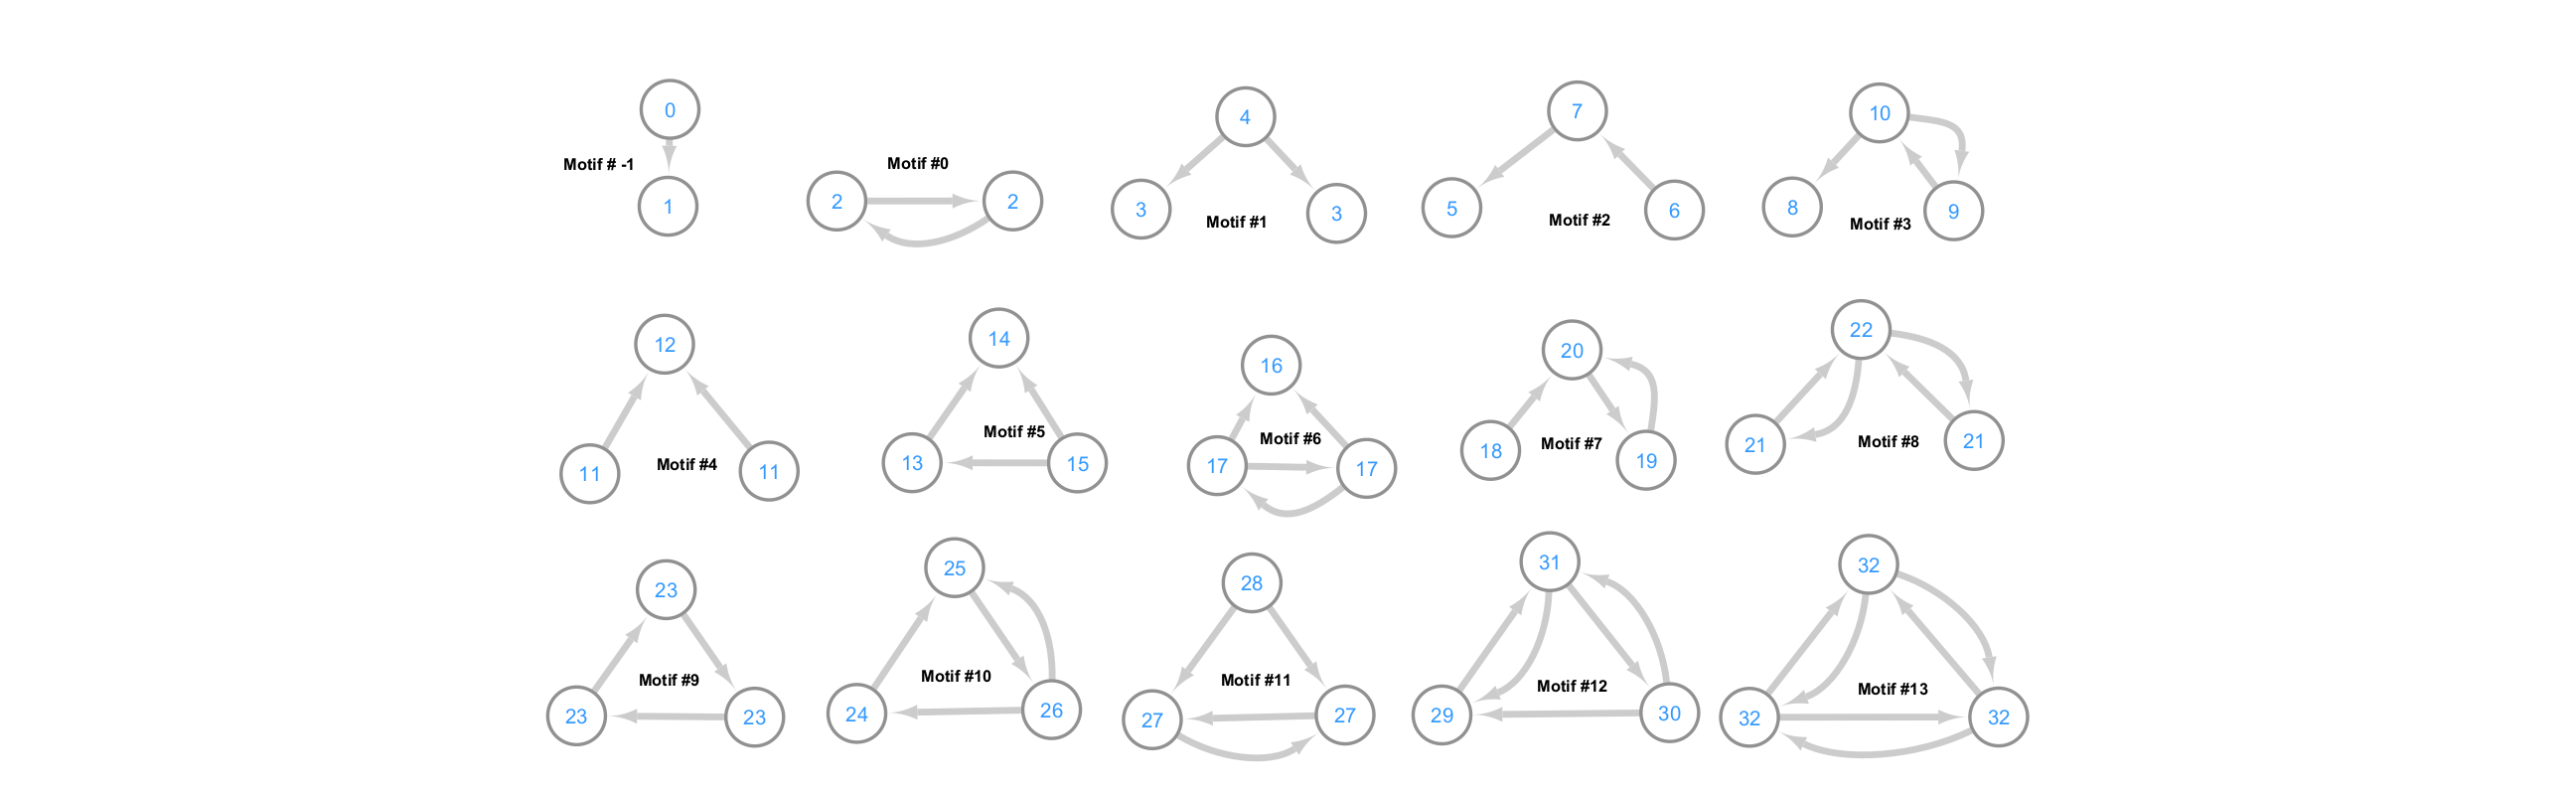
\includegraphics[width=\linewidth]{motifs.png}
	\caption{The generated directed motif atlas, denoting all possible induced subgraph types of sizes 2 and 3. The nodes are labelled with the 33 possible orbital roles.}
	\label{fig:motifs}
\end{figure}

\begin{figure}[t]\centering
	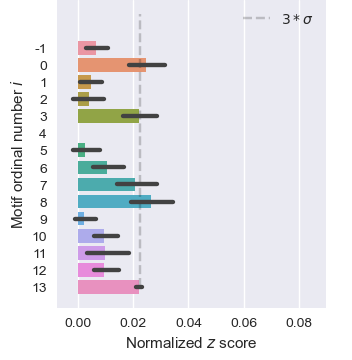
\includegraphics[width=\linewidth]{generalimportance.png}
	\caption{Overal motif significances show that motifs }
	\label{fig:GeneralSignificance}
\end{figure}

\begin{figure}[t]\centering
	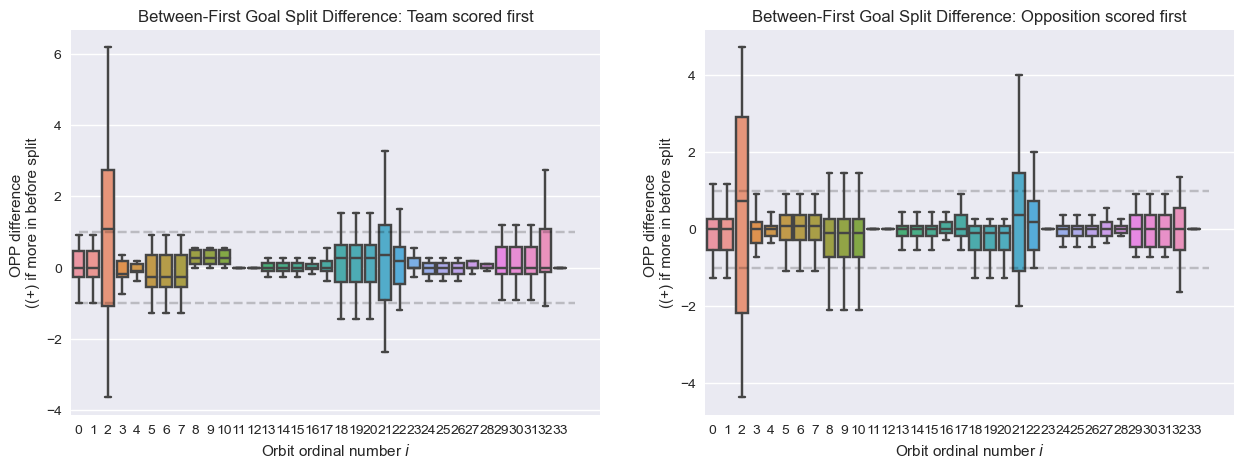
\includegraphics[width=\linewidth]{OrbitGoals.png}
	\caption{Overal motif significances show that motifs }
	\label{fig:OrbitsGoals}
\end{figure}


\begin{figure}[t]\centering
	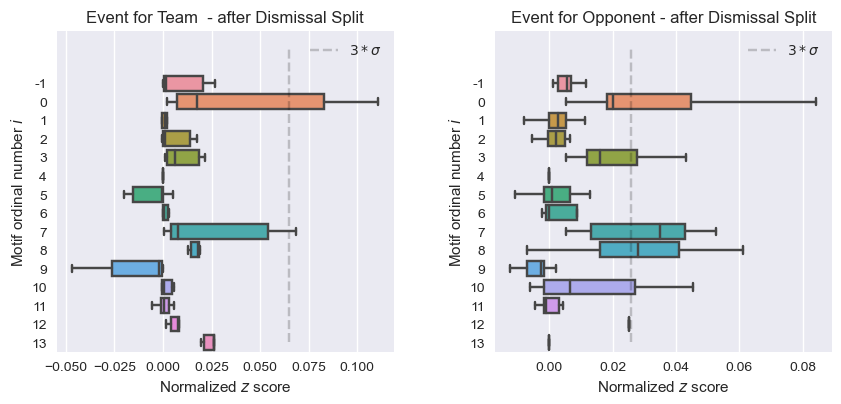
\includegraphics[width=\linewidth]{MotifSignificanceDismissal.png}
	\caption{Overal motif significances show that motifs }
	\label{fig:MotifSignificanceDismissal}
\end{figure}





\section*{Discussion}


\begin{figure}[t]\centering
	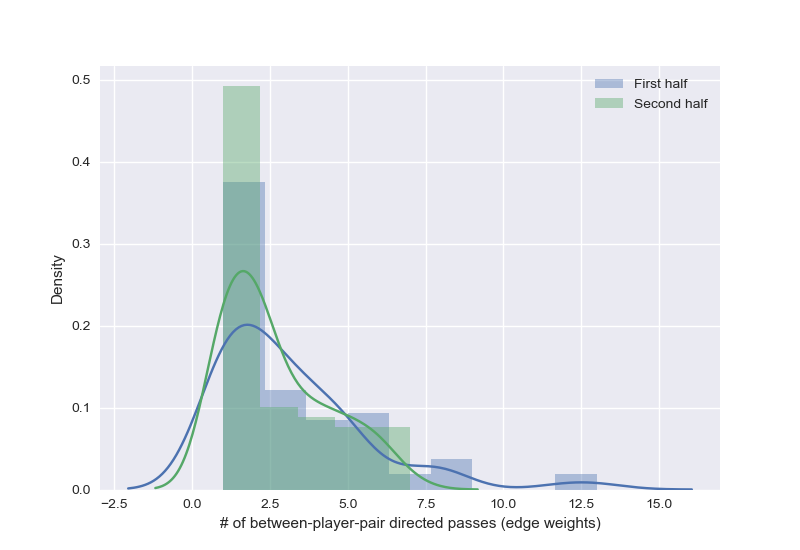
\includegraphics[width=0.8\linewidth]{BayernPassWeightComparison.png}
	\caption{The distribution of graph edge weights in Bayern Münich's 2012 Champions league final loss versus Chelsea shows that edge weights roughly follow a Poisson distribution. As the same trends emerge in other examined games as well, we note that pruning the graphs at just above the median $\floor{\lambda + \frac{1}{3} - \frac{0.02}{\lambda}} \approx \lambda$ will result in considering only the non-trivial passes, carrying information about frequent passes of play.}
	\label{fig:BayernWeights}
\end{figure}
{\small\section*{Methods}

{\bf All of the described results were achieved by analysing directed networks with player-nodes and weighted pass edges, with weights corresponding to pass frequency.} 

\subsection*{Data}
All of the examined networks were parsed from alternative data structes by Statsbomb \cite{statsbomb}. Unless noted otherwise, the described results were achieved by aggregating the findings of analyses, conducted on 789 parsed matches. For each successful pass, a directed edge was generated between the players, logged in the corresponing pass attempt and reception events, logged by the data provider. For the three considered key events - the half time break, the first goal and the first dismissal in any given match, 6 directed \textit{pajek} files were created for each involved team (3 before and 3 after the key event), where games without certain events contain empty \textit{after-event} files. Additionally, the graphs' flow centrality variants were created and saved according to the procedure, described in the following subsection. For the calculation of network intensity, the description of which also follows, the team posession time was calculated as  the sum of timestamp differences in each uninterrupted posession stint.

\subsection*{Centrality and intensity}
\subsection*{Communities}
\subsection*{Network fragments}
In all experiments concerning network fragments, the networks were pruned before examination. This was done by removing all edges with weights equal to or less than the median weight from the observed graph. The estimation of an adequate pruning point stems from the insights, described in the caption of Figure \ref{fig:BayernWeights}.

To examine the orbit-representation in the observed graphs, an atlas of all possible directed graphlets of node-count 3 or less was created. From there, each unique edge subset from the analysed graph was extracted and a hash table of benchmark orbital roles created. For each subgraph, inferred from the edge subsets, the orbital roles for each contributing node were calculated. The resulting table of this procedure denoted the number of occurences of each player in each of the 34 considered orbital roles. Each network's orbital profile is then calculated as the average number of player-occurences in each orbital role, divided by 11 - the number of players on the pitch. By comparing the differences between these profiles before and after key events, the final insights of the distrbution of OPP (orbit-occurences per player) differences is achieved.
Similarly, the induced motifs were also initially counted by detecting isomorphisms between fixed-size subgraphs and graphlets from the atlas. In an approach described in \cite{przulj}, the significance of each motif is calculated by comparing the number of its occurences to that expected in a directed configuration model, corresponding to the considered graph's in and out degree. In our approach, 100 different configuration models are created to compute these expected values. From there, the motif significance profile for motif $i$ is calculated as shown in Equations \ref{eq:1}.



\begin{equation}
SP_{i} = \frac{Z_{i}}{\sqrt{\sum_{i}{Z_{i}^{2}}}} = \frac{\frac{n_{i} - E[\tilde{n}_{i}]}{\tilde{\sigma}_{i}}}{\sqrt{\sum_{i}{(\frac{n_{i} - E[\tilde{n}_{i}]}{\tilde{\sigma}_{i}})^{2}}}} \label{eq:1},
\end{equation} where $n$ is the number of motif occurences, $\tilde{\sigma}$ is the standard error of all empiric configuration graph observations of $\tilde{n}$, the number of motif occurences in the configuration model.


\acknow{The authors would like to acknowledge the help of Doc.  Dr. Lovro Šubelj in the identification of feasible problems within our domain of interest for this course project and for all the help offered in solving them.}

\showacknow{}

\bibliography{bibliography}

\end{document}